Sections~\ref{sec:feature_salience}~and~\ref{sec:deep_learning_salience}
have focused on identifying the most important content for summary inclusion,
while punting somewhat on summary generation -- and for good reason, 
extractive summarization minimizes the burden of creating fluent text. 
While abstractive text generation certainly adds significant challenges to 
summary creation, 
its benefits are many: the ability to achieve tighter compression ratios
for space constrained scenarios \citep{fan2017controllable}, the potential
to target different reading levels \citep{margarido2008automatic}
or style \citep{shen2017style}, and more pragmatically, in
an increasingly copy-protected web, abstractive generation may be the only 
legally viable option for content aggregation services 
\citep{kassam2014google}.

With this expressive power comes the danger that the generated text may
misconstrue the source material. Trust in machine learning
models is increasingly being recognized as an important factor in user 
adoption \citep{ribeiro2016should}, and mistakes of this kind will be 
a show stopper for downstream consumers of summarization (e.g. if an
abstractive summarization model in the previous crisis-monitoring scenario
erroneously attributes the location of a deadly earthquake). 

\begin{figure}
 \centering
 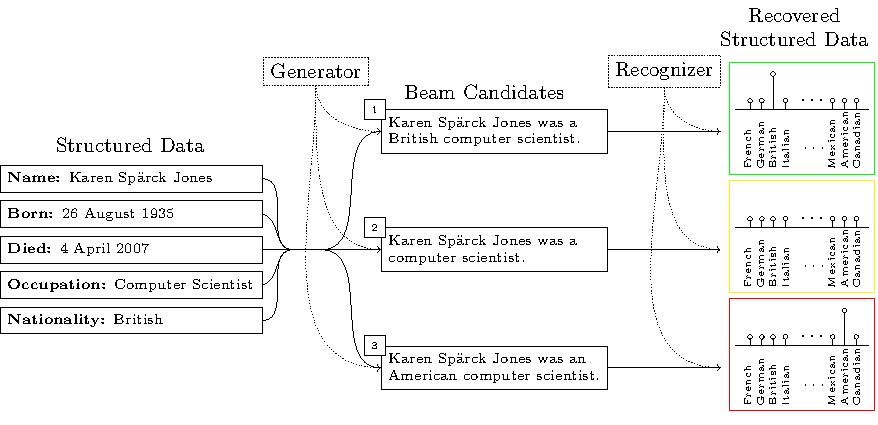
\includegraphics{images/faithful_generation/example1.pdf}
 \caption{Example of faithful generation from structured data. The generator
 is responsible for producing a list (beam) of candidate utterances from the 
 structured data. The recognizer reranks the beam candidates based on the 
 plausibility of the recovered structured data. }
 \label{fig:fgen_example1}
\end{figure}


As a potential solution,
we propose modeling text generation as a two player game between a generator
model and a recognizer model. %, akin to an auto-encoder \citep{rumelhart1985learning}. 
First, we provide as input to the 
generator some evidence (e.g., raw text or table data). 
Conditioned on the evidence, the generator must produce 
a list of candidate utterances accurately describing that evidence. The recognizer
scores the candidates based on its ability to reconstruct various 
pieces of the evidence. The generator receives supervision in the form of a 
reference utterance (i.e. standard sequence maximum likelihood training) 
and also from the recognizer scores across all candidate
utterances.
I.e., the generator learns to produce a variety of utterances that are
simultaneously fluent but also lead the recognizer to recover the original
evidence correctly. If we have an accurate recognizer, the generator should
improve in its ability to render truthful descriptions of the evidence.



% no alignments needed
% decompose supervision into fluency and truthfulness
% learn mutliple realizations that are fluent and correct.
% can experiment in controllable generation 
% can experiment with different soft constraints


There are several motivations for this approach. 
First, RNNs typically used to implement text generators are impressive
conditional language models and will generally learn to create fluent outputs.
By adding a faithfulness component (recognizer derived 
losses) to the learning objective we can hopefully improve reliability 
of text generation for downstream users. 

Second, by learning across
multiple (beam search) candidates, we can encourage the model to 
explore syntactically and lexically diverse paraphrases that are still
factually licensed by the evidence. We think this will be usefull when
text generation is part of a pipeline that may want to consider various 
realizations to ensure fluency and coherency at a macro, e.g. document, level.

Furthermore, the recognizer is itself a learned model; 
as text classification models improve, so will the faithful generation 
framework.
It does not require
alignments between the evidence and the reference utterances; it uses
the same evidence/utterance parallel data as the generator to train.
The recognizer can also be used to derive confidence scores 
for individual utterances if this is needed
in a downstream application. 


Finally, we think this framework also allows for an alternative approach
to controllable text generation. Currently, most controllable approaches
to generation rely on appending feature embeddings to the decoder 
input (e.g. for length \citep{fan2017controllable} or for syntactic 
structure \citep{colin2018generating}). By specifying a desired output from
the recognizer, we can train biased generators that adhere to soft constraints,
similar to these other methods.
What's more, the recognizer allows us to certify that individual outputs 
actually adhere to the desired constraints, something the input only control
mechanisms do not do.



%First we do not need 
%alignments between the evidence and the utterances, the recognizer can learn
%from 



%~\\
%~\\

%While we will experiment with a variety of loss functions to find something
%that works well empirically, we expect in principal to train the generator
%to maximize the expected likelihood of evidence under the recognizer.



See \autoref{fig:fgen_example1} for an example 
where we have table data as evidence (biographical data about name, nationality, and 
occupation), and we generate several plausible and implausible 
candidates that are evaluated by the recognizer.
The first candidate is 
 ranked highly because the recognizer can correctly infer that the 
 nationality of Karen Sp\"arck Jones is British (green box). The second 
 candidate is possibly fine because it maximizes entropy over the choice 
 of nationalies (yellow box), i.e. it makes no commitments either way and does
 not produce a non-true statement. The third beam candidate is clearly wrong
 as the recognizer infers that the nationality is American which is a false
 statement according to the true table data (red box).
 In some applications it may be OK to omit information, in which case the first
 and second utterances are acceptable and we only want to train the generator to
 avoid the third. In other cases, we may want to require that all input
 evidence has some corresponding description in the output, in which case,
 only the first utterance is acceptable. 
 The faithful generation framework allows us to learn what the correct possible outputs are  
 by specifying which recognizer distributions are acceptable. 

In the remainder of this section, we cover the related work in this area
before describing in more detail the faithful generation framework for 
data-to-text and text-to-text scenarios and our proposed experiments.
%formally define two faithful generation
%models, one for generating text from structured data and 
%one for generating text from  text data. We conclude by briefly describing some
%applications and datasets we will use to evaluate these modls.

\subsection{Related Work}

%In our proposed faithful generation framework, we use one model, the 
%generator, to
%create a text utterance, e.g. a summary of a document or a description
%of a data table, and another model, the recognizer, to answer questions 
%about the underlying document or table, using the utterance as evidence.
%A good utterance, then, is one that allows the recognizer on average to
%correctly answer those questions.

The conceptual underpinnings of faithful generation trace back to two
ideas in the NLP literature. The first is round-tripping in machine translation
\citep{somers2005round,rapp2009back}, i.e. a good translation system should be able to translate
a source language text to a target language text and then back to the source
language with minimal corruption between the original source and the 
back-translated source. \cite{andreas2016reasoning} have recently carried 
this idea 
over to explaining structured prediction tasks, where, e.g., 
the structure is a 
formal plan for a robotic agent; a rational speaker  generates the text
description of the plan that is most likely to lead a rational listener 
to correctly re-interpret the original plan. Faithful generation is similar:
the generator (speaker) 
 encodes an 
input object
(either text or data table) into 
an intermediate text representation, and the recognizer (listener) then tries to 
answer questions about the source using only the intermediate text.
The main difference is that in faithful generation, we are interested not in
a full reconstruction of the source from the intermediate representation, but
rather, the utility of the intermediate representation on a downstream task, 
e.g. question answering.


The other conceptual precedent is that of discriminative reranking 
of $n$-best lists \citep{collins2005discriminative,charniak2005coarse};
a generative model produces the $n$ most likely latent structures, e.g. parses,
and a discriminative model, which does not have the burden of modeling
the observations, rescores this list.  This idea has been applied 
to text generation as well. \cite{wen2015stochastic} and 
\cite{novikova2017e2e} use a 
sequence-to-sequence
model with beam search to generate $n$-best texts from either a 
dialogue plan or data table respectively,
 and then use a separately trained
classifier to downrank the beam candidates that do not correspond to the 
underlying
structured object.
%statements (according to the data table).
We argue that this is insufficient since we might want to consider 
all beam candidates in a downstream task, e.g. a macro content planner stage.
%that maximizes the  coherency of a sequence generated utterances.
For this model to provide linguistically interesting realizations that are 
still
factually true requires expanding the beam size 
which increases the computational and memory demands at test time. 
In our faithful generation framework, we directly discourage the generator from
ever allowing an untrue statement to be kept in the beam. This is done
using the recognizer directly as a learning signal and backpropagating
through the beam search process \citep{wiseman2016sequence}.

Increasingly, summarization researchers are exploring
 \textsc{Reinforce}-style
policy gradient methods to optimize non-differentiable metrics like 
\textsc{Rouge} \citep{paulus2017deep,arumae2018reinforced,kryscinski2018improving,narayan2018ranking,pasunuru2018multi}.
The most related to our work is that of \cite{arumae2018reinforced} 
and \cite{pasunuru2018multi}.
\cite{arumae2018reinforced} 
learn an extractive summarization model that maximizes
performance of a question-answering model on cloze style questions created
from the reference summaries. In our proposed method, the questions are 
generated from the source document and we use abstractively generated 
summaries as
the input to the question answering model, a significantly harder task.
\cite{pasunuru2018multi} learn an abstractive summarization model that
optimizes the likelihood that the generated summary is entailed by the 
ground-truth reference summary. The entailment likelihood is obtained from a
model trained on the SNLI \citep{bowman2015large} and MULTI-NLI 
\citep{williams2018broad} datasets.
This entailment measure is somewhat orthogonal to the faithful generation 
objective, as our proposed
approach directly evaluates the utility of the summary as a faithful proxy
for the underlying document, not the reference, which is the ultimate goal of the 
summarization task.


Most reinforcement learning applied to abstractive summarization uses
one Monte-Carlo sample from their policy distribution to estimate the 
expected reward. We propose to optimize
the entire beam search so that all beam candidates are viable in downstream
tasks. In this way, faithful generation also resembles 
minimum error rate training (MERT) \citep{och2003minimum} 
and minimum Bayes-risk decoding (MBD)
\citep{kumar2004minimum} in that we are reshaping a distribution of $n$-best
beam candidates to optimize the expected value of an evaluation metric.
We also plan on using reward shaping supervision from the recognizer
model to localize reward signals \citep{mnih2014neural} to specific spans of 
a candidate utterance
that are most responsible for violating the input document. Localized
reward shaping will help to penalize only the factually incorrect spans
and preserve syntactic and structural choices that are independent of 
such entailment considerations.


Other notable approaches to improving the faithfulness of abstractive 
generation include \cite{guo2018soft} who use a multi-task training objective 
to learn a shared decoder that can alternatively summarize a document,
generate a question about a document, or generate a logically entailed text 
from a document.
The latter task is relevant here, as the authors claim that this entailment
generation objective encourages the decoder to produce only logically entailed
summaries. This claim deserves further scrutiny as their human 
evaluation only asked about \textit{relevance} and \textit{fluency} where
the relevance criteria included topical relevance and redundancy in addition
to factual accuracy, confounding any interpretation of the generated summaries
as being more faithful to the source document.

%~\\
%This is done by learning from 
%Our proposed method is to learn from the recognizer's signals
%during training, i.e. backpropagating throught the beam search process
%so that the beam does not need to to be pruned during test time, i.e. 
%all surviving beam 
%candidates should be factually true.



%Similarly, minimum error rate training (MERT) \citep{och2003minimum} 
%and minimum Bayes-risk decoding 
%\citep{kumar2004minimum}
%rerank $n$-best translations in order to directly optimize an evaluation
%metric like \textsc{Bleu} \citep{papineni2002bleu}.

%Faithiful generation can be recast in the MERT framework by considering
%the evaluation metric to be the recognizer's classification accuracy on
%table data or cloze accuracy on text data. This is perhaps most similar
%to    


